\documentclass{beamer}
\usetheme{Warsaw}
\setbeamertemplate{headline}{}
\graphicspath{ {./images/} }
\usepackage{amsmath}


\usepackage{amssymb}
\usepackage{algpseudocode}
\usepackage{algorithm}
\usepackage{setspace}
\usepackage{graphicx}
\graphicspath{ {./images/} }
\usepackage{hyperref}
\usepackage{siunitx}
\usepackage{amsmath}
\usepackage{caption}
\usepackage{subcaption}

\title[Binding affinity prediction of PL complexes using ML]{Binding Affinity Prediction of Protein-Ligand complexes using Machine Learning}

\author[Abdus Salam Khazi]
{
    \textbf{MSc Project}\\
    Abdus Salam Khazi
}

\institute{Supervisors: \\
            \begin{tabular}{ll}
		    	Simon Bray \& Alireza Khanteymoori
		    \end{tabular}
}

\date{\today}
\logo{
\includegraphics[width=.2\textwidth]{Logo}}

\hypersetup{
    colorlinks=false,
    linkcolor=blue,
    filecolor=magenta,      
    urlcolor=cyan,
}

\begin{document}

\begin{frame}
\titlepage
\end{frame}

\begin{frame}{Table of Contents}
\tableofcontents
\end{frame}

\section{Introduction}

\subsection{Biological Background}

\begin{frame}[t]{Biological Background}
What are a proteins and ligands? 
\begin{itemize}
\item \textbf{Proteins:} Complex molecules that are work-horses (machines) of a living organism.
\item \textbf{Ligands:} Molecules that bind to particular proteins, called receptor proteins.

\item Proteins and ligands bind together to form protein-ligand complexes.

\end{itemize}

\begin{figure}[htb]
  \centering
    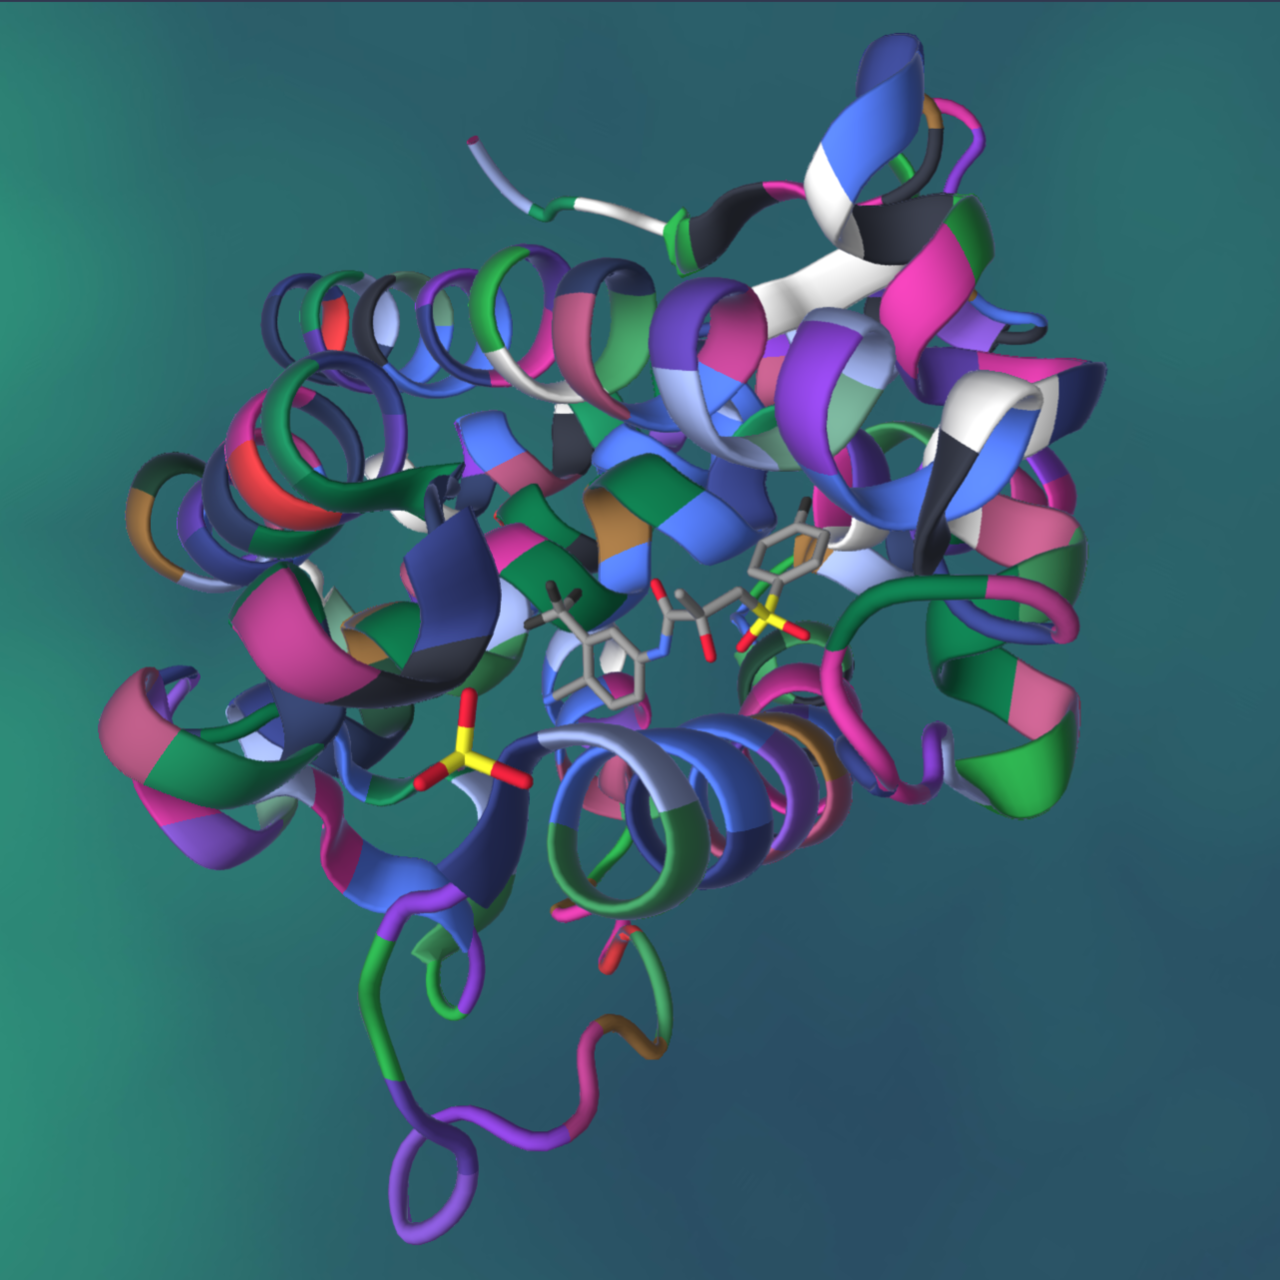
\includegraphics[scale=0.07]{images/pl_complex}
    \caption{Haemoglobin transporter protein \cite{PL_complex_introduction}.}
    \label{fig:HaemoglobinTransporterImage}
\end{figure}

\end{frame}

\begin{frame}[t]{Biological Background}
Protein-Ligand complexes

\begin{itemize}
\item Any potential binding location in the 3D structure of a protein is called a
pocket.
\item The pockets of proteins only bind to ligands of complementary shape.
\item Drugs are just ligand molecules that bind to protein to cause a therapeutic effect.
\end{itemize}

\begin{figure}[htb]
  \centering
    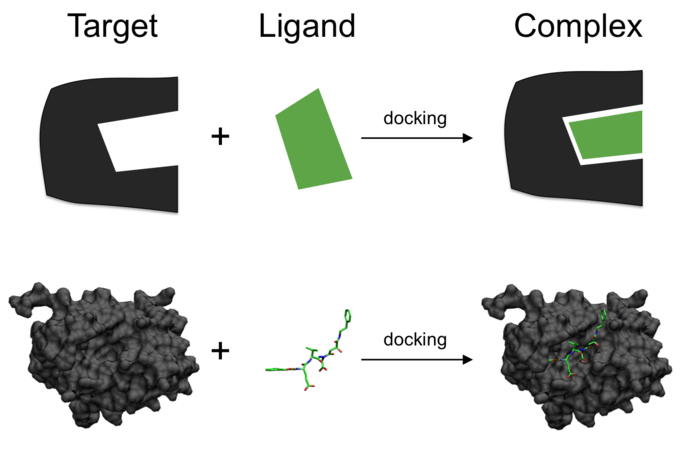
\includegraphics[scale=0.45]{images/lock_and_key}
    \caption{Lock and Key hypothesis in molecular docking \cite{lockandkeyformatpng}.}
    \label{fig:lockandkey}
\end{figure}


\end{frame}

\begin{frame}[t]{Biological Background}
Understanding Protein-Binding Affinity.

\begin{itemize}
\item Binding affinity between a protein and a ligand is quantified by the $K_d$, $K_i$ and $IC_{50}$.
Here $K_d$ refers to the dissociation constant, $K_i$ to inhibition constant, and $IC_{50}$ to 
inhibitory concentration 50\%.
\item $K_d$ can be quantified by using protein concentration $[P]$ and ligand concentration $[L]$ at equillibrium \cite{proteinlingandbindingpaper}.
$$K_d = \frac{[P][L]}{[PL]}$$
\item $K_i$ and $IC_{50}$ are similarly defined.
\end{itemize}


\end{frame}

\subsection{Problem Definition.}

\begin{frame}[t]{Problem Definition}

\begin{itemize}
\item Determining if a potential drug (ligand) can bind to a target protein is very costly processes \cite{drugdiscoverycost}.
\item The project aims to predict the ligand affinity based on previously recorded data ("In-Silico" method).  This reduces the drug discovery costs.
\item We use PDB databank,  which holds PL affinity data collected over many decades.
\end{itemize}

\begin{figure}[htb]
  \centering
    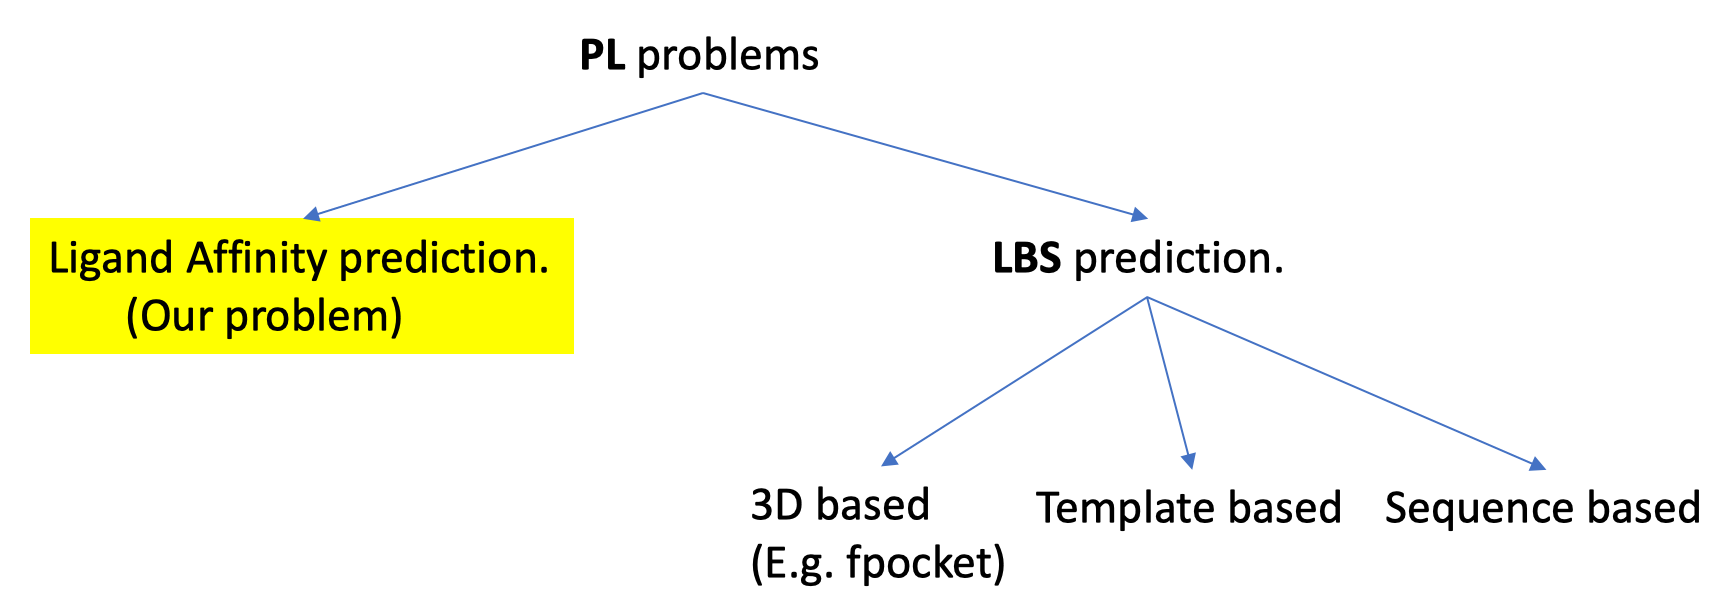
\includegraphics[scale=0.25]{images/pl_problem_classification}
    \caption{Protein-Ligand problem classifcation.}
    \label{fig:plproblemclassification}
\end{figure}


\end{frame}

\section{Methods}
\subsection{Feature Extraction}

\begin{frame}[t]{Feature Extraction}
\textbf{PDB databank} (v2019) was used to extract input features.
\begin{itemize}
\item We use \textit{fpocket/dpocket} ligand binding site prediction library to get the features of pockets pockets in proteins.
\item \textit{RDKit} library is used to extract features for each ligand.
\item \textbf{Ligand Features:} Using \textit{RDKit.Chem.Descriptors}, $402$ features were extracted for each ligand.  Hence the ligand features space was $\mathbf{R}^{402}$.
\item \textbf{Protein Features:} For every pocket,  55 descriptors are obtained in total. Hence, the input space for protein features is $\mathbf{R}^{55}$
\end{itemize}
The concatinated input feature space before input feature elimination $\mathbf{R}^{457}$.

\end{frame}

\subsection{Feature Selection}

\begin{frame}[t]{Feature Selection}
We only had $16000$ data points to train a feature space of $\mathbf{R}^{457}$. 
We reduced our features using the following feature selection strategies:
\begin{itemize}
\item \textbf{Output Correlation}: The input features that have the best \textit{Pearson} and \textit{Spearman} correlation were selected. \cite{spearmanpearsoncorrelation}.
\item \textbf{Genetic Algorithms}: Genetic algorithms with the following score function was used to select the best features \cite{geneticalgorithmsresearchpaper}:
$$
\textrm{score} = \mathbf{R}^2 \textrm{score} * \textrm{Features Eliminated}
$$
\item \textbf{Manual Feature Selection:} A selected list of 121 ligand descriptors was
used with all protein descriptors as input to the model.
\end{itemize} 
\end{frame}

\subsection{Testing strategy}

\begin{frame}[t]{Testing strategy}
We use the following methods to determine the quality of results and reproducing them:
\begin{itemize}
\item \textbf{Reproducibility}: To reproduce the results, we use report random seed (Execution ID) for every execution. 
\item \textbf{$R^2$ score} (\textit{Coefficient of determination}) \cite{r_squared_score}: . $R^2  \in (- \infty, 1.0]$ where $1.0$ is the best score. 
\item \textbf{Visualization:}
Our model's approximated function $ f : \mathbf{R}^n \mapsto \mathbf{R} \;\; \textrm{where} \;\; n \in \mathbf{I}^+$ is visualized as a 2D scatter plot.

\begin{figure}[htb]
  \centering
    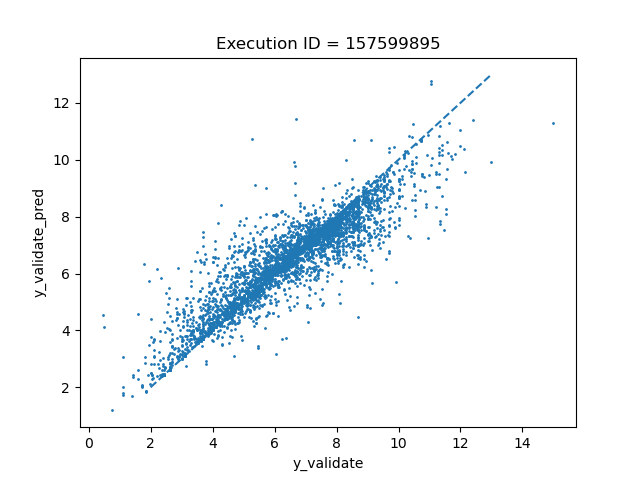
\includegraphics[width=0.40\textwidth]{images/accuracy_validate}
    \caption{(Sample) Visualizing accuracy.  $R^2 \approx 0.805$.}
    \label{fig:modelQualityVisualization}
\end{figure}

\end{itemize} 
\end{frame}

\subsection{Data preprocessing}

\begin{frame}[t]{Data Preprocessing}
\begin{itemize}
\item Anomalies such as NaN (Not a number) values were removed from the data before sending them as input to the model.
\item We used PCA (principle component analysis) to find that the ligand feature \textit{IPC} was having log scale values.
\end{itemize}

\begin{figure}
     \centering
     \begin{subfigure}[b]{0.4\textwidth}
         \centering
    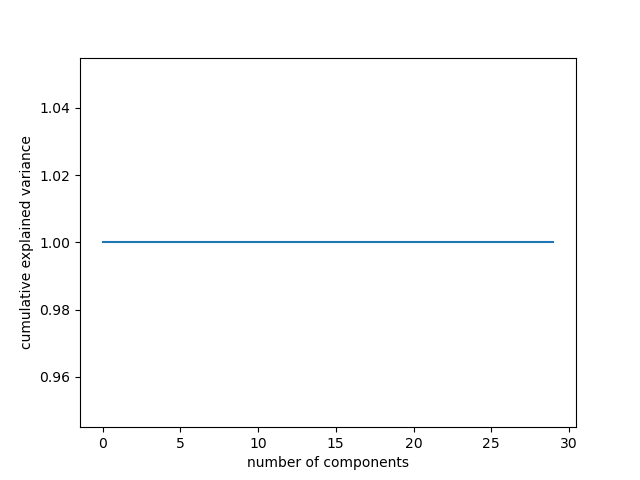
\includegraphics[scale=0.25]{images/pcaligandanalysisIPC}
    \caption{With original Ligand feature IPC.}
    \label{fig:pcaproteinanalysisIPC}
     \end{subfigure}
     \hfill
     \begin{subfigure}[b]{0.4\textwidth}
         \centering
        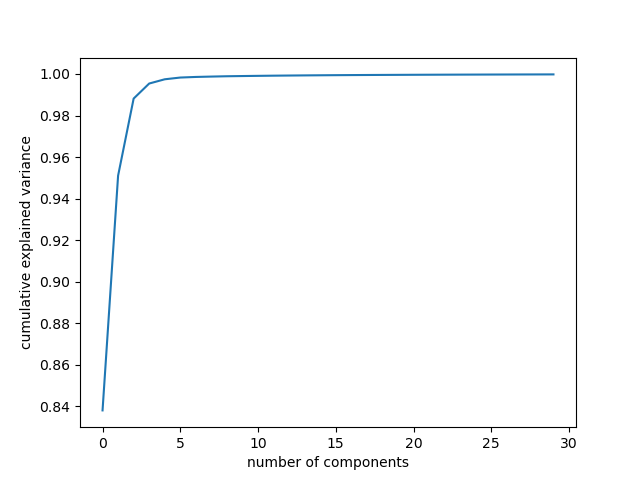
\includegraphics[scale=0.25]{images/pcawithscaledIPC}
        \caption{With log scaled Ligand feature IPC.}
        \label{fig:pcawithscaledIPC}
     \end{subfigure}
     \caption{Cumulative PCA of ligand features.}
     \label{fig:PCAAnalysis}
\end{figure}

\end{frame}


\begin{frame}[t]{Dealing with measurement resolution}
\begin{itemize}
\item In the PDB databank,  each complex also has a corresponding measurement resolution.
\item The structural
detail of the 3D image is inversely proportional to the measurement
resolution.
\item The weighting of each data point was done according to hyperbolic formulae and linear formulae.
$  W_i = \frac{ \mathrm{\max{R_{1 ...  n}}}}{R_i}  ;  W_i = (\mathrm{\max{R_{1 ...  n}}} + 1) - R_i $
\end{itemize}

\begin{figure}
     \centering
         \centering
    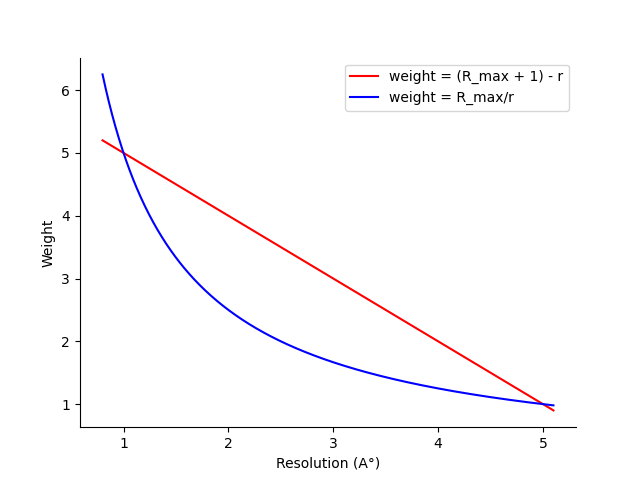
\includegraphics[scale=0.3]{images/graphingformula}
    \caption{Weight calculation formulae.}
    \label{fig:graphingformula}
\end{figure}

\end{frame}


\section{Q \& A}

\begin{frame}[t]{Q \& A}
  \centering \Huge
  \emph{Q \& A}
\end{frame}

\section{References}

\begin{frame}[t]{References}

\begin{thebibliography}{1}

\bibitem{proteinlingandbindingpaper}
\alert{Du,  Li,  Xia,  Ai,  Liang,  Sang,  Ji and Liu; Insights into Protein–Ligand Interactions: Mechanisms, Models, and Methods (2016)}

\bibitem{drugdiscoverycost}
\alert{DiMasi,  Grabowski and Hansen; nnovation in the pharmaceutical industry: New estimates of R \& D costs (2016)}

\bibitem{r_squared_score}
\alert{scikit-learn; R2 score, the coefficient of determination},

\bibitem{geneticalgorithmsresearchpaper}
\alert{John H. Holland.  Genetic Algorithms. (1960)}

\bibitem{spearmanpearsoncorrelation}
\alert{Schober, Boer and Schwarte. Correlation Coefficients: Appropriate Use and Interpretation. (2018)}

\bibitem{PL_complex_introduction}
\alert{Protein–Ligand complex; Wikipedia.}

\bibitem{lockandkeyformatpng}
\alert{Docking (molecular); Wikipedia.}

\end{thebibliography}

\end{frame}

\end{document}
